\section{Methods}
\label{sec:methods}

\subsection{用于提取密集特征和扩大感受野的空洞卷积}
\label{sec:convnet-hole}

DCNNs 用于语义分割或其他密集预测任务已被证明可以通过以完全卷积形式简单而成功地解决 \cite{sermanet2013overfeat, long2014fully}。然而,这些网络中最大池化层和跳跃层的重复组合显著地降低了所得特征图的分辨率,最近的 DCNNs 中通常降低了 32 倍。部分补救方法是使用 `反卷积' 层 \cite{long2014fully},但这需要额外的时间与内存。 

我们主张使用空洞卷积,最初是为了在 ``algorithme \`a trous'' 中高效计算未抽取的小波变换而开发的 \cite{holschneider1989real, giusti2013fast, sermanet2013overfeat, papandreou2014untangling}。该算法允许我们以任何所需的分辨率计算任何层的响应。一旦网络经过训练,它就可以在事后部署应用,也可以与训练无缝集成。

先考虑一维信号,空洞卷积 \footnote{我们遵循 DCNN 文献中的标准实践,并在此定义中使用非镜像滤波器。} 的输入是 $x[i]$,输出是 $y[i]$,滤波器是长度为 $K$ 的 $w[k]$,定义如下:
\begin{equation}
  y[i] = \sum_{k=1}^K x[i + r \cdot k] w[k].
\end{equation}
上式中的 $r$ 是步长,与采样率有关。标准卷积是 $r=1$ 时的特例,参见 \figref{fig:hole}。

\begin{figure}
  \begin{tabular}{c}
    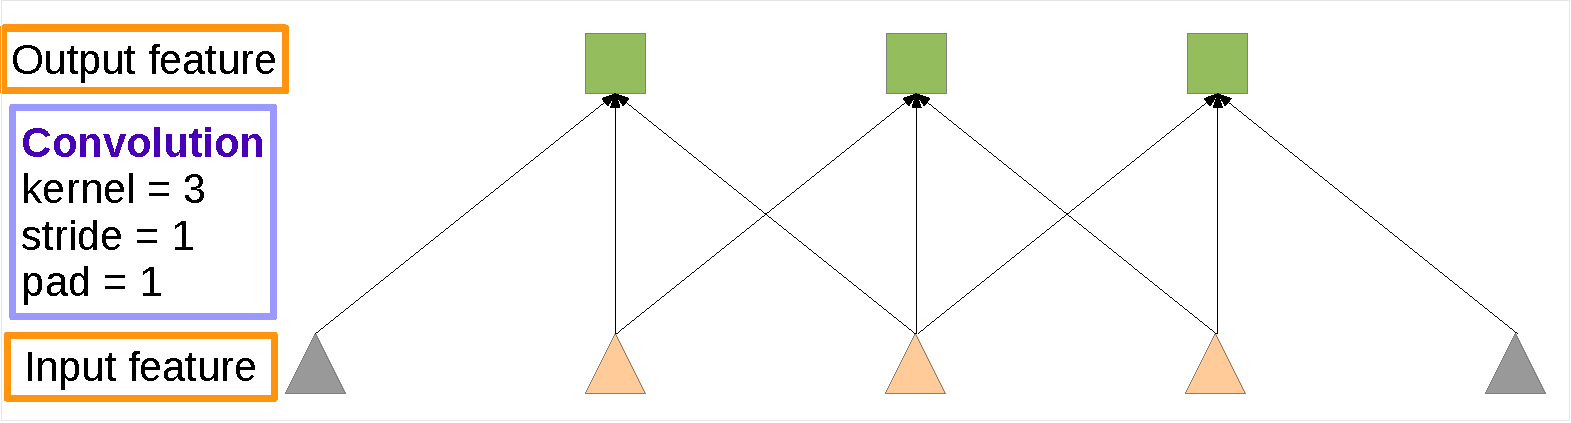
\includegraphics[width=0.9\linewidth]{fig/atrous_fig1.pdf} \\
    {\scriptsize (a) 稀疏特征提取} \\
    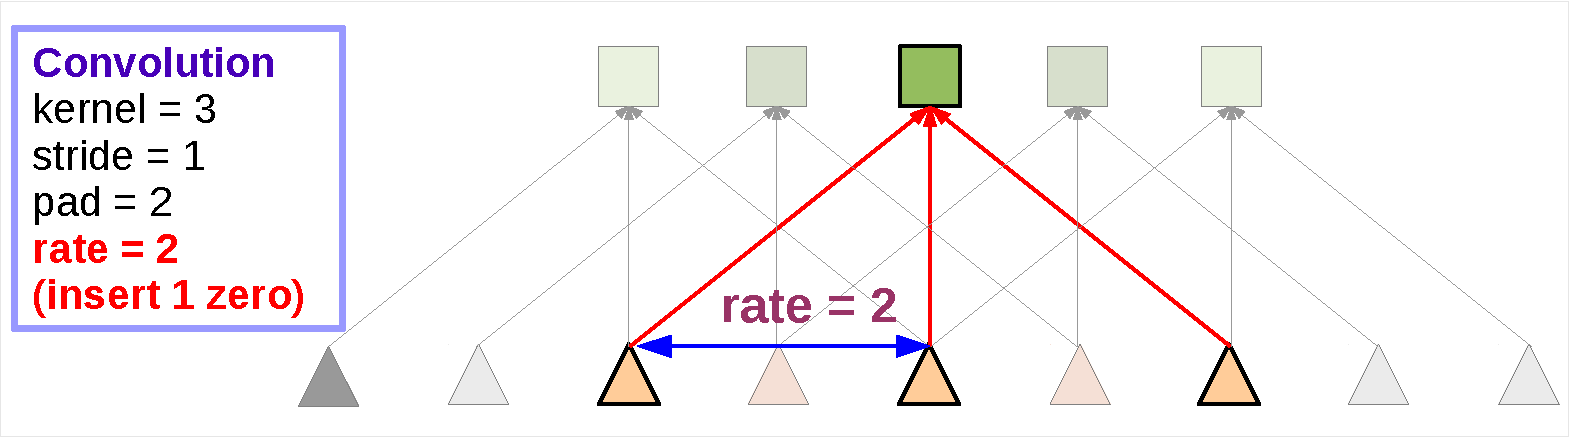
\includegraphics[width=0.9\linewidth]{fig/atrous_fig2.pdf} \\
    {\scriptsize (b) 密集特征提取} \\
  \end{tabular}
  \caption{一维空洞卷积计算图示。(a) 在低分辨率输入特征图上使用标准卷积进行稀疏特征提取。
    (b) 在高分辨率输入特征图上使用 $r=2$ 的空洞卷积进行密集特征提取。}
  \label{fig:hole}
\end{figure}

我们通过 \figref{fig:hole2d} 中的一个简单示例来说明算法在二维输入上的操作:给定输入图像,我们假设首先进行下采样操作,将分辨率降低两倍,然后使用垂直高斯导数卷积核进行卷积运算。如果在原始图像坐标中植入生成的特征图,我们意识到仅在原始图像位置的 1/4 处获得了特征响应。相反,如果我们将原始分辨率图像与空洞卷积滤波器进行卷积,可以计算出所有图像位置的响应,其中我们将原始滤波器上采样两倍,并在滤波器值之间置入 0。虽然滤波器尺寸增加,但是仅仅只要计算非零的位置,因此滤波器参数的数量和每个位置的操作数量保持不变。此方案允许我们容易且明确地控制神经网络特征响应的分辨率。

\begin{figure}
  \centering
  \begin{tabular}{c}
   	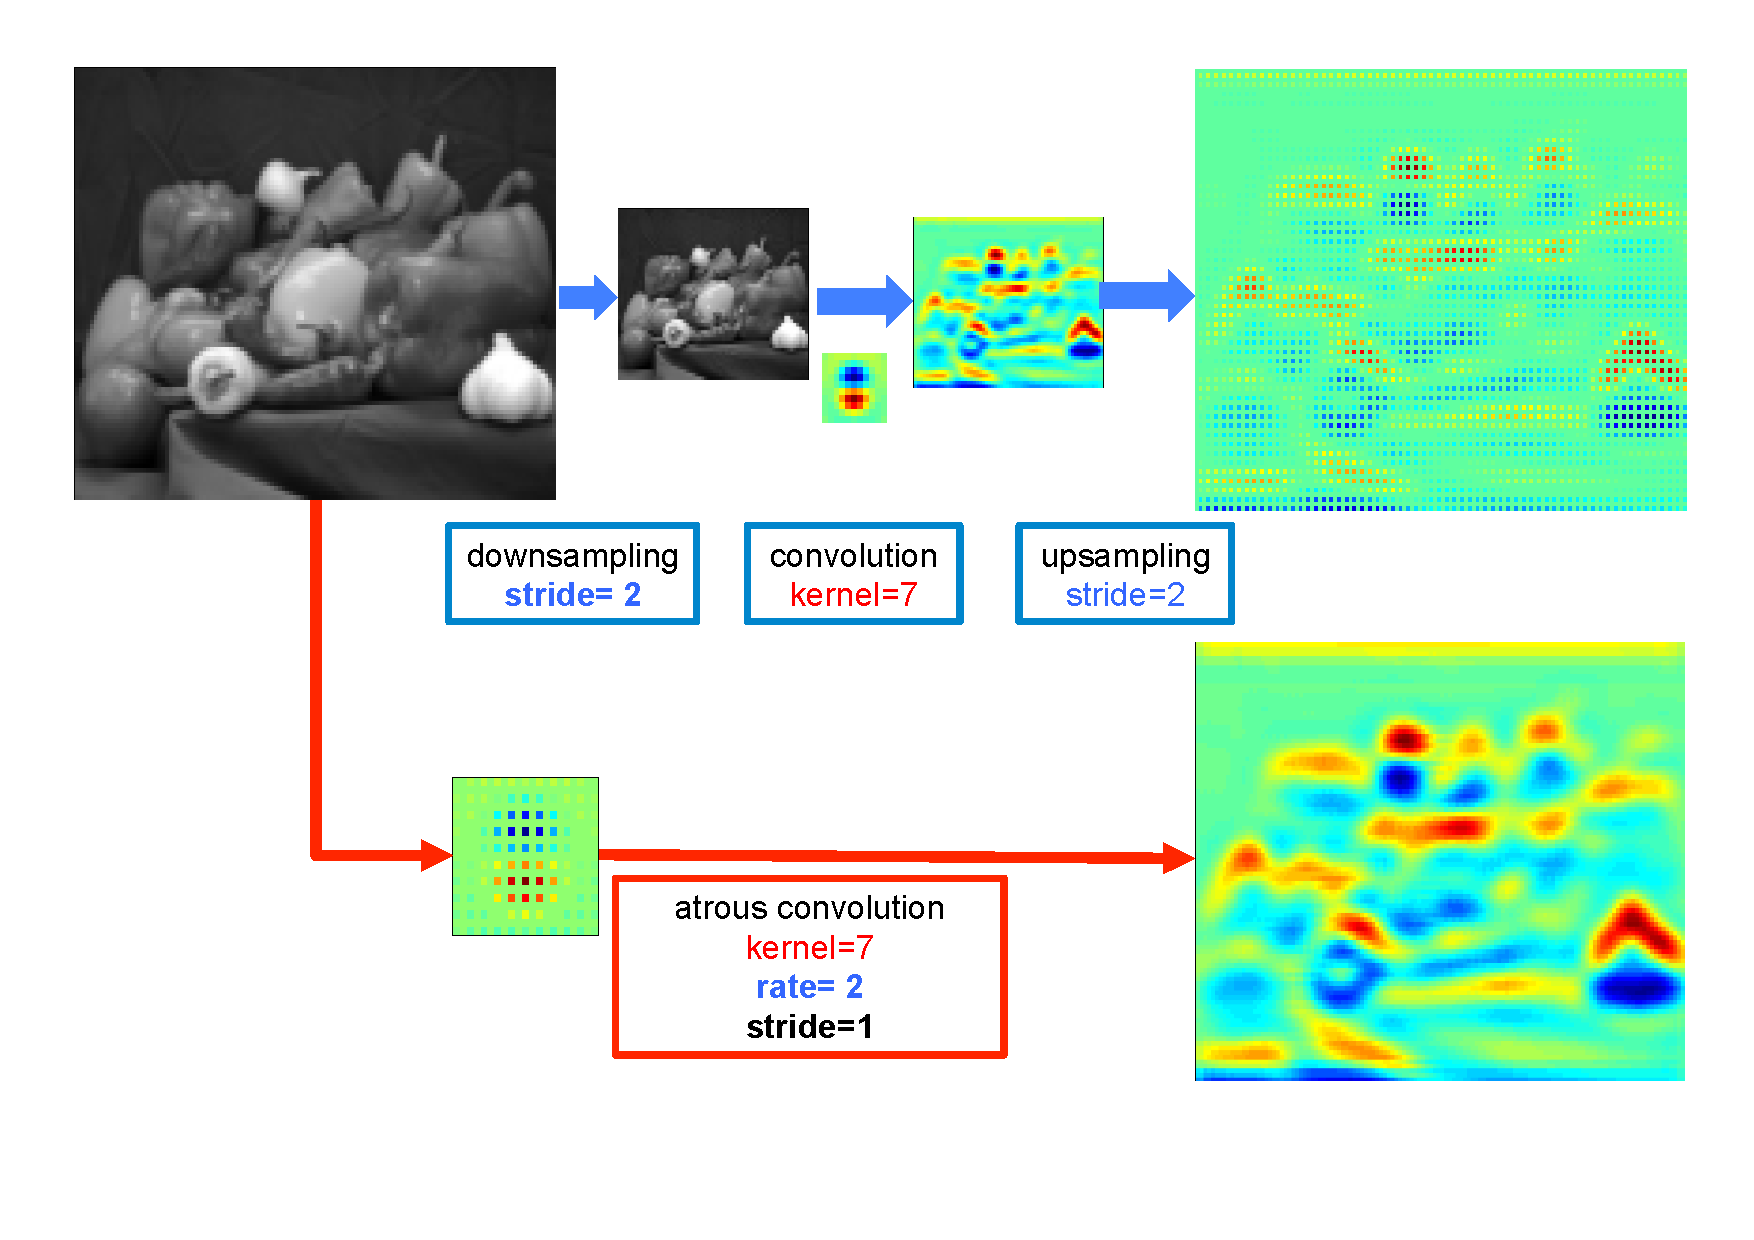
\includegraphics[width=.99 \linewidth]{fig/atrous_slide_rate.pdf}
   	\vspace{-.9cm}
  \end{tabular}
  \caption{二维空洞卷积计算图示。上图:在低分辨率输入特征图上使用标准卷积进行稀疏特征提取。下图:在高分辨率输入特征图上使用 $r=2$ 的空洞卷积进行密集特征提取。}\label{fig:hole2d}
\end{figure}

在 DCNNs 中,我们可以使用空洞卷积层以任意分辨率计算最终的特征响应。例如,为了使 VGG-16 或 ResNet-101 网络中计算出的特征响应的分辨率加倍,我们将最后一个降低分辨率的池化层或卷积层(分别为 `pool5' 和 `conv5\_1')的步长设为 1 避免信号抽取,并通过使用 $r=2$ 的空洞卷积层替换后续所有卷积层。通过这种方法我们可以以原始图像分辨率计算特征响应,但这成本略高。我们采用了一种混合方法,该方法可以实现良好的效率/准确性权衡,使用空洞卷积将计算特征图的分辨率增加 4 倍,然后通过额外因子 8 快速双线性插值来恢复特征图分辨率。双线性插值在此情境下表现足够好,因为分类得分图(对应于分类对数概率)非常平滑,如 \figref{fig:score-maps} 所示。与 \cite{long2014fully} 中的反卷积方法不同的是,我们提出的方法将图像分类网络转化为更为密集特征提取器,而无需学习任何额外的参数,从而在实践中实现更快的 DCNN 训练。

空洞卷积还允许我们在任何 DCNN 层上任意放大滤波器的 \textit{感受野}。最先进的 DCNN 通常使用较小的卷积核(通常是 \by{3}{3}),以便保证较少的参数量。而使用扩张率为 $r$ 的空洞卷积在连续的滤波值之间插入 $r-1$ 个 0,有效地将 \by{k}{k} 的滤波器大小扩大到了 $k_e = k + (k-1)(r-1)$ 而无需增加参数量或计算量。因此,它提供了一种有效的机制来控制感受野,并找到精确定位(小感受野)与上下文同化(大感受野)之间的最佳平衡。我们已经成功地尝试了这种技术:我们的 DeepLab-LargeFOV 模型变体 \cite{chen2014semantic} 在 VGG-16 的 `fc6' 层中使用了 $r=12$ 的空洞卷积,显著地提升了性能,详见第~\ref{sec:experiments}~章。

在实现方面,有两种有效的方法来实现空洞卷积。第一种是通过插入孔(0)来隐式地对滤波器进行上采样,或者等效地稀疏地对输入特征图进行采样 \cite{holschneider1989real}。我们在早期的工作中实现了这个 \cite{papandreou2014untangling, chen2014semantic}。之后,Caffe 框架 \cite{jia2014caffe} 给稀疏采样过程添加了 \textsl{im2col} 函数(它从多通道特征图中抽取向量化的像素)\cite{yu2015multi}。第二种方法是在 \cite{shensa1992discrete} 中提出,并在 \cite{giusti2013fast, sermanet2013overfeat} 中使用的。它对输入特征图进行子采样,其采样因子为空洞卷积的 $r$,产生了降低 $r^2$ 分辨率的特征图,每一个对应原图中的 \by{r}{r} 的可能偏移。然后将标准卷积应用于这些中间特征图并将它们重新偏移出原始图像分辨率。通过将空洞卷积减少为常规卷积,它允许我们使用现成的高度优化的卷积框架。我们已经在 TensorFlow 框架中实现了第二种方法 \cite{abadi2016tensorflow}。

\subsection{使用空洞空间金字塔池化的多尺度图像表示}

DCNNs 已经表现出显著的隐式表达比例变化的能力,只需在包含不同大小的物体的数据集上进行训练即可。尽管如此,明确物体的大小规模可以提高 DCNNs 处理大型和小型物体的能力 \cite{papandreou2014untangling}。

我们已经尝试了两种处理语义分割中的尺度可变性的方法。第一种相当于标准的多尺度处理 \cite{chen2015attention, kokkinos2016pushing}。我们使用共享参数的并行 DCNNs 从多个重新缩放版本的图像数据集中提取 DCNN 得分图(我们使用了 3 个数据集)。为了产生最终结果,我们将并行DCNN分支的特征映射双线性插值到原始图像分辨率并融合它们,通过在每个位置获取不同尺度上的最大响应。在训练与测试阶段我们都是这么做的。多尺度处理显着提高了性能,但代价是在 DCNNs 的所有层上都要计算特征响应以用于多种输入规模。

第二种方法的灵感来自于 \cite{he2014spatial} 的 R-CNN 空间金字塔池化方法的成功应用,其表明通过重新采样在单一尺度上提取的卷积特征,可以准确且有效地对任意尺度的区域进行分类。我们已经实现了他们方案的变体,其使用具有不同采样率的多个并行的空洞卷积层。针对每个采样率提取的特征在单独的分支中进一步处理并融合以生成最终结果。我们提出的 ``空洞空间金字塔池化''(DeepLab-ASPP)方法概括了 DeepLab-LargeFOV 变体,参见 \figref{fig:aspp_fov}。

\begin{figure}[!t]
  \centering
  \scalebox{1}{
  \begin{tabular}{c}
    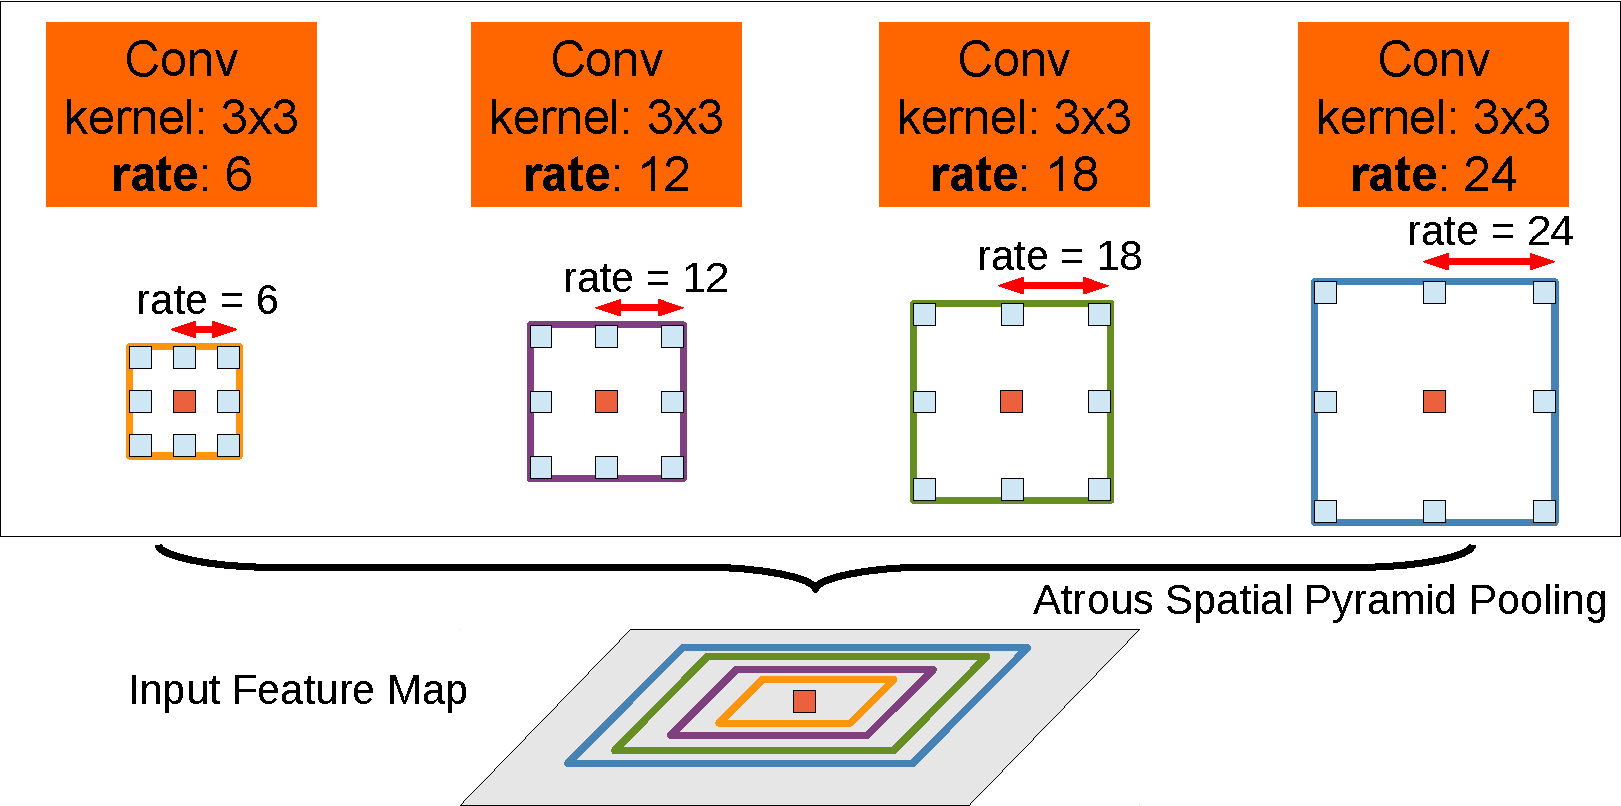
\includegraphics[height=4.5cm]{./fig/spm/aspp2.pdf} \\
  \end{tabular}
  }
  \caption{空洞空间金字塔池化(ASPP)。为了对中心像素(橙色)进行分类,ASPP通过采用具有不同 $r$ 的多个并行滤波器来利用多尺度特征。有效的视野以不同的颜色显示。}
  \label{fig:aspp_fov}
\end{figure}

\subsection{基于全连通条件随机场的用于精确边界恢复的结构预测}
\label{sec:boundary-recovery}

定位精度与分类精度之间的权衡似乎是 DCNNs 中固有的常态:具有多个最大池化层的深度模型已经证明在分类任务中表现最为出色,但顶层节点增加的不变性与大型的感受野只能产生平滑的特征响应。如 \figref{fig:score-maps} 中所示,DCNN 得分图可以预测物体的存在以及大致的位置,但是无法准确描述其边界。

以前的研究主要追求两方面来解决这一定位挑战。第一种方法是利用卷积网络中多个层的信息,以便更好地估计物体边界 \cite{hariharan2014hypercolumns, long2014fully, eigen2014predicting}。第二种方法是采用超分辨率表示,基本上将定位任务委派给了低级的分割方法 \cite{mostajabi2014feedforward}。

我们结合 DCNNs 的识别能力和全连接 CRF 的细粒度定位精度来替代传统方法。实验表明,基于 DCNNs 与 全连接 CRF 的模型在解决定位问题上非常成功,产生了准确的语义分割结果,并且在一定程度上恢复了物体的边界,其细节处理远远超过了现有的方法。由于本工作第一个版本的发表 \cite{chen2014semantic},之后的几篇论文也推广了这个方向 \cite{papandreou2015weakly, schwing2015fully, zheng2015conditional, dai2015boxsup, noh2015learning, liu2015semantic, lin2015efficient, chen2015attention, chen2015semantic}。

\begin{figure}[t]
  \centering
  \begin{tabular}{ccccc}
    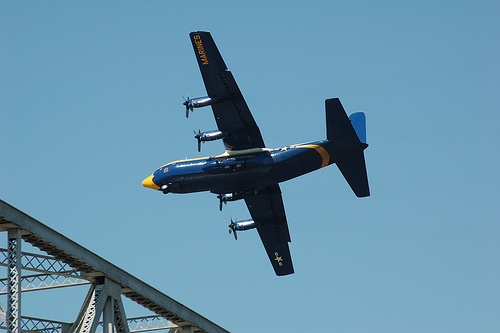
\includegraphics[width=0.16\linewidth]{fig/mean_field_illustration/2007_007470.jpg} & 
    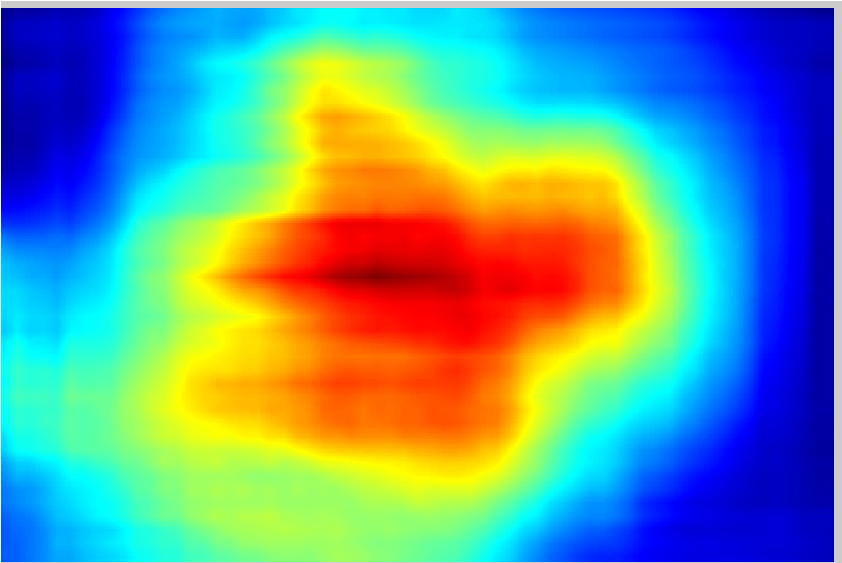
\includegraphics[width=0.16\linewidth]{fig/mean_field_illustration/Score_Class1_Itr0.pdf} &
    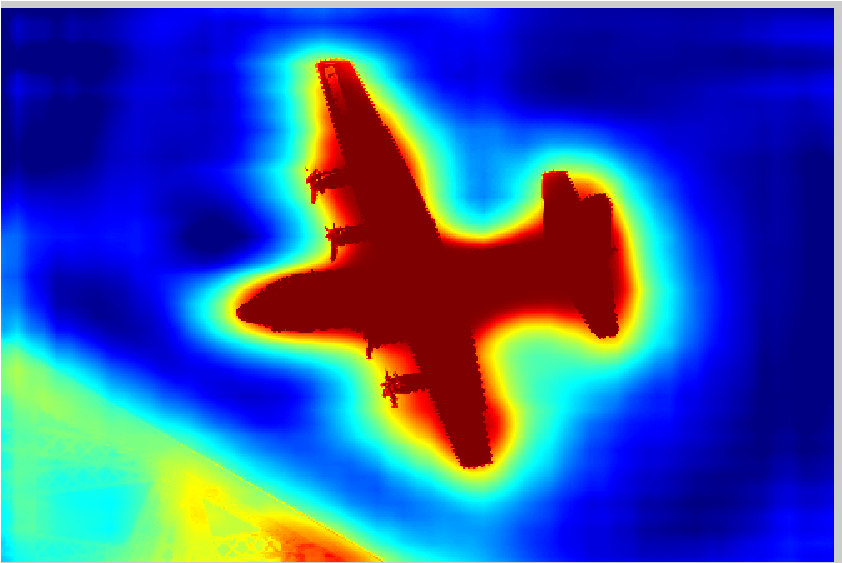
\includegraphics[width=0.16\linewidth]{fig/mean_field_illustration/Score_Class1_Itr1.pdf} & 
    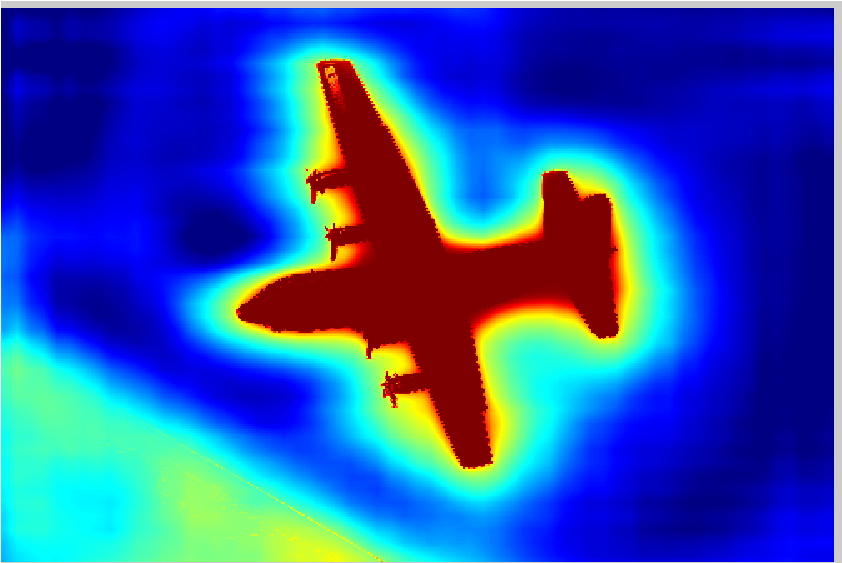
\includegraphics[width=0.16\linewidth]{fig/mean_field_illustration/Score_Class1_Itr2.pdf} & 
    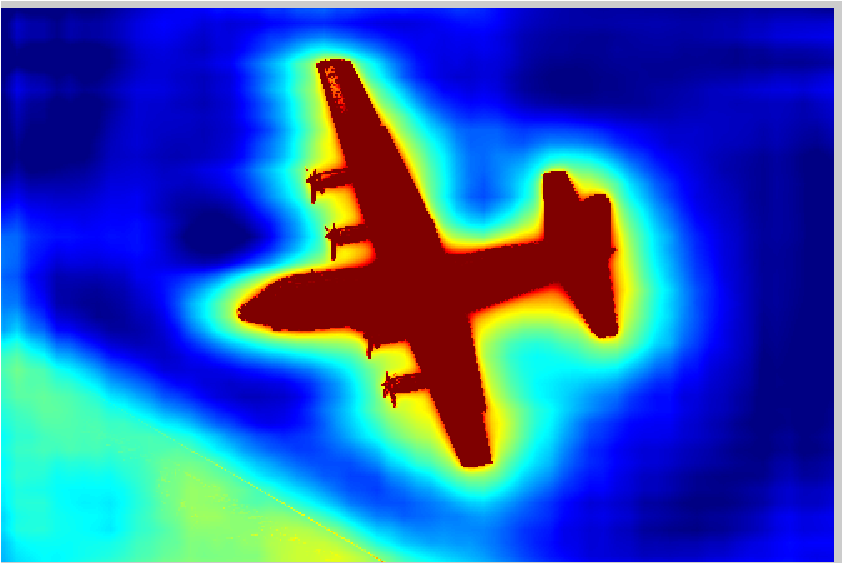
\includegraphics[width=0.16\linewidth]{fig/mean_field_illustration/Score_Class1_Itr10.pdf} \\
    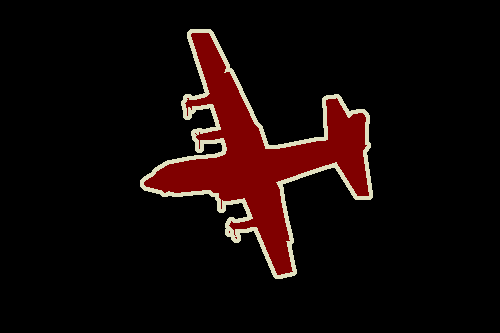
\includegraphics[width=0.16\linewidth]{fig/mean_field_illustration/2007_007470.png} & 
    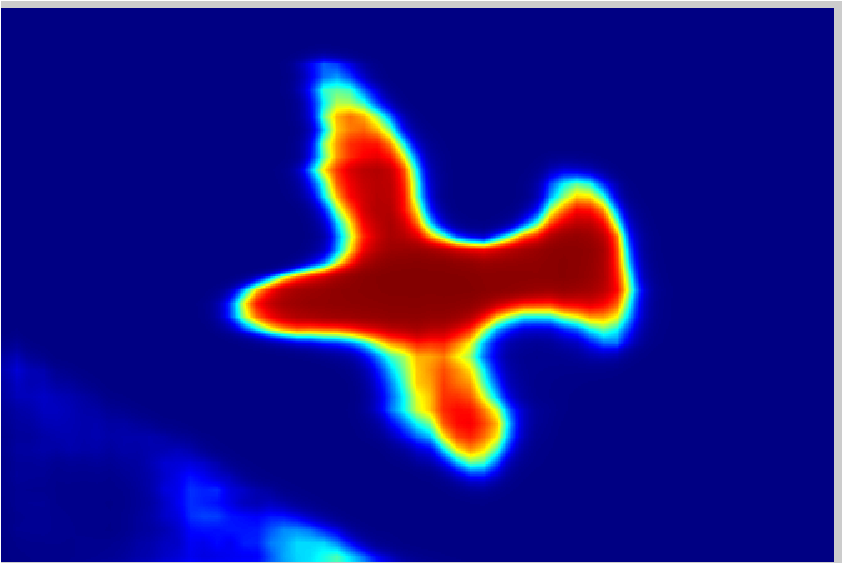
\includegraphics[width=0.16\linewidth]{fig/mean_field_illustration/Belief_Class1_Itr0.pdf} & 
    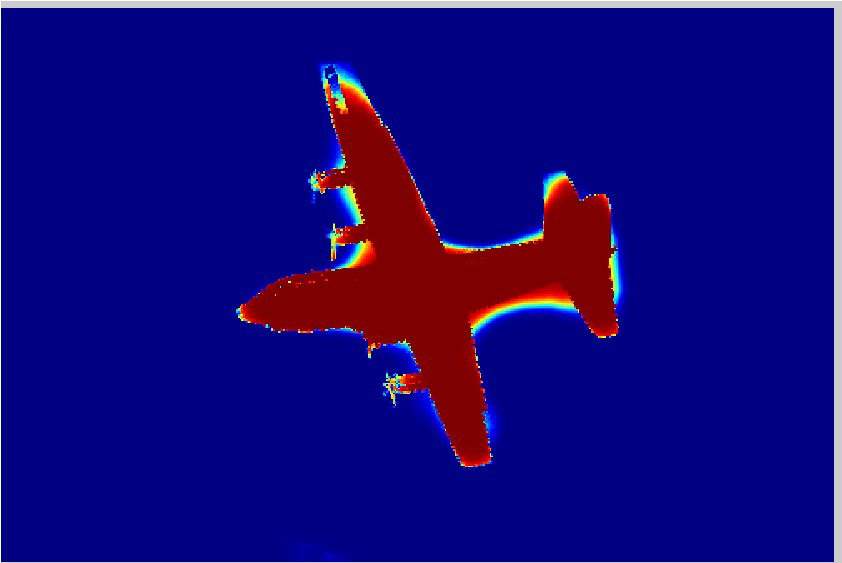
\includegraphics[width=0.16\linewidth]{fig/mean_field_illustration/Belief_Class1_Itr1.pdf} & 
    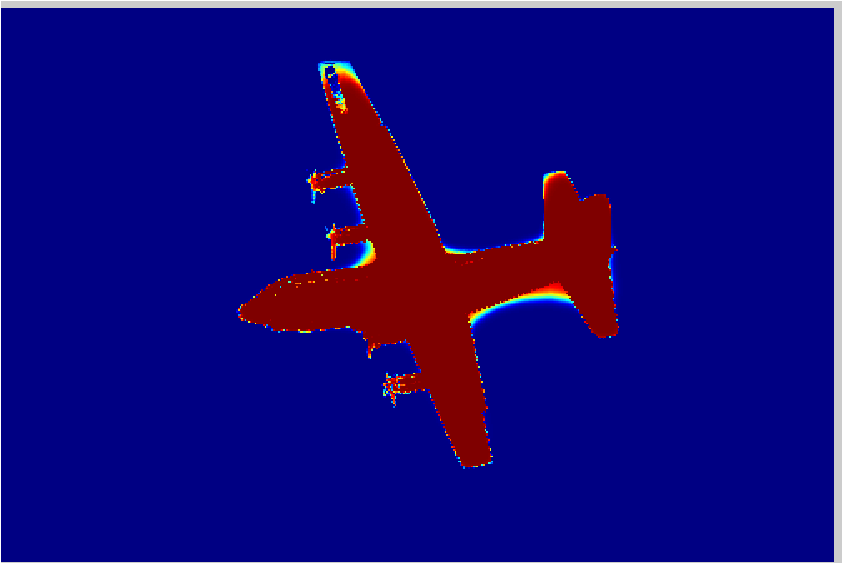
\includegraphics[width=0.16\linewidth]{fig/mean_field_illustration/Belief_Class1_Itr2.pdf} & 
    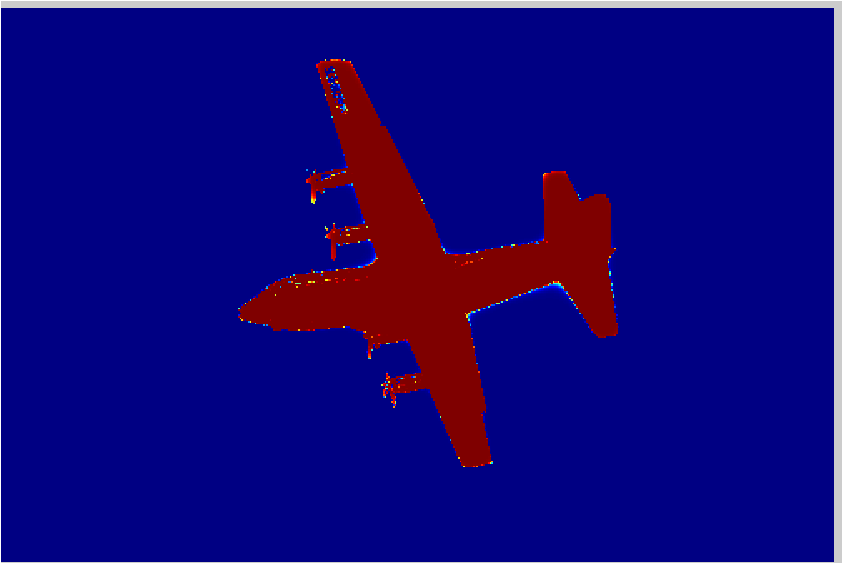
\includegraphics[width=0.16\linewidth]{fig/mean_field_illustration/Belief_Class1_Itr10.pdf} \\
    {\tiny Image/G.T.} & {\tiny DCNN output} & {\tiny CRF Iteration 1} & {\tiny CRF Iteration 2} & {\tiny CRF Iteration 10} \\
  \end{tabular}
  \caption{预测为飞机的得分图(未经过 softmax)与 概率图 (经过 softmax)。我们在每次平均场迭代后记录得分(第一行)与概率(第二行)。最后一个 DCNN 层的输出用作平均场推断的输入。}
  \label{fig:score-maps}
\end{figure}

传统上,条件随机场(CRF)已用于平滑噪声分割图 \cite{rother2004grabcut, kohli2009robust}。通常,这些模型将相邻节点结合,有利于相同标签分配到空间上临近的像素。定性地说,这些短距离的 CRFs 是为了清理人工特征构建的弱分类器所产生的虚假预测。

与传统的弱分类器相比,现代 DCNN 结构(例如我们在此工作中使用的结构)产生的得分图与语义标签预测有着质的飞跃。如 \figref{fig:score-maps} 所示,得分图通常十分平滑,且产生同质分类结果。在这种情况下,使用短程的 CRFs 可能是有害的,因为我们的目标是恢复详细的分类结果而非进一步地平滑它。结合对比敏感势能 \cite{rother2004grabcut} 与局部范围的 CRFs,可以潜在地改善定位,但依然缺少轻量结构,通常需要解决更难的离散优化问题。

为了克服短程 CRFs 的这些限制,我们将全连接的 CRFs 模型 \cite{krahenbuhl2011efficient} 整合进来。该模型采用能量函数
\begin{align}
  E(\boldsymbol{x}) = \sum_i \theta_i(x_i) + \sum_{ij} \theta_{ij}(x_i, x_j)
\end{align}
其中 $\boldsymbol{x}$ 是像素的标签。我们使用 DCNN 计算出的一元势能 $\theta_i(x_i) = - \log P(x_i)$,其中 $P(x_i)$ 是像素标签概率。成对势能允许在使用全连通图时,即在连接所有图像像素对 $i,j$ 时进行有效的推断。我们引用 \cite{krahenbuhl2011efficient},将其表达为以下形式:
\begin{gather}
  \hspace{-.2cm}\theta_{ij}(x_i, x_j) \!=\! \mu(x_i,x_j)\!\left[w_1 \exp \Big(\!-\!\frac{||p_i-p_j||^2}{2\sigma_\alpha^2} \!-\!\frac{||I_i-I_j||^2}{2\sigma_\beta^2}\! \Big)\right. \nonumber\\
  \left. + w_2 \exp \Big(-\frac{||p_i-p_j||^2}{2\sigma_\gamma^2}\Big)\right]\label{eq:fully_crf}
\end{gather}
其中,当 $x_i \neq x_j$ 时 $\mu(x_i,x_j)= 1$,$x_i = x_j$ 时,$\mu(x_i, x_j)=0$,在 Potts 模型中,这表示只有具有不同标签节点才会受到惩罚。其他表达式在不同的特征空间中使用两个不同的高斯核; 第一个``双边''核取决于像素位置(表示为$ p $)和 RGB 颜色(表示为$ I $),第二个仅取决于像素位置。超参数 $\sigma_\alpha, \sigma_\beta, \sigma_\gamma$ 控制了高斯核的缩放比例。第一个核强制那些有相似颜色和位置的像素有相似的标签,而第二个核仅在强制平滑时考虑空间接近度。

值得注意的是,这个模型适用于有效的近似概率推理 \cite{krahenbuhl2011efficient}。在完全可分解的平均场近似值 $b(\boldsymbol{x}) = \prod_i b_i(x_i)$ 下传递更新的消息可以表示为双边空间中的高斯卷积。高维滤波算法 \cite{adams2010fast} 显著加快了这一计算速度,从而使算法在实践工程中非常快。当使用开源的 \cite{krahenbuhl2011efficient} 时,Pascal VOC 数据集中的图像平均推断时间不到 0.5 秒。
